\documentclass[10pt]{beamer}

\usetheme[language=italian,
  titlepagelogo=logo_unisalento,
  bullet=triangle,
  color=green,
  pageofpages=di,
  titleline=true
  ]{TorinoTh}

\author{Mosè Giordano}
\rel{Achille Nucita}
\title{Il problema dei due corpi e applicazioni astrofisiche}
\institute[UniSalento]{Università del Salento}
\date{20 ottobre 2011}

\usefonttheme{professionalfonts}
\usepackage{lxfonts}

\usepackage{booktabs,siunitx,tikz,tikz-3dplot,pgfplots}
\pgfplotsset{compat=1.3}

\usepackage[font=scriptsize,format=hang,labelformat=empty,
textformat=period]{caption}

\sisetup{per-mode=symbol,
  inter-unit-separator={}\cdot{},
  exponent-product=\cdot,
  output-product=\cdot,
  separate-uncertainty=true
}

\graphicspath{{Immagini/}} % cartella in cui cercare le immagini da caricare
\setbeamercovered{dynamic} % rende il testo coperto trasparente in modo
                           % dinamico: la trasparenza sarà tanto più marcata
                           % quanto più tempo il testo dovrà rimanere coperto, e
                           % viceversa.

% ridefinisco i comandi per alcune lettere greche in modo che si usino le
% varianti
\renewcommand{\phi}{\varphi}
\renewcommand{\epsilon}{\varepsilon}

%% Nuove unità di misura
\DeclareSIUnit\parsec{pc}
\DeclareSIUnit\year{yr}
\DeclareSIUnit\solarmass{\ensuremath{M_\odot}}
% C'era già l'arcosecondo, però lo ridefinisco per essere coerente con gli
% articoli che cito
\DeclareSIUnit\arcsecond{as}

% definisco il comando `\bm' uguale a `\vec' perché nelle slide preferisco
% mettere la frecce piuttosto che usare il grassetto. Non uso direttamente
% sempre `\vec' perché includo una figura tikz (momento_angolare.tex) che non
% posso/voglio modificare e utilizza `\bm'.
\newcommand{\bm}[1]{\vec{#1}}

%%%%% Funzioni PGF
% funzione che restituisce la distanza dal fuoco di un punto di un'ellisse in
% corrispondenza dell'anomalia vera #1 (\e = eccentricità, \p = semilato retto)
\pgfmathdeclarefunction{dist}{1}{\pgfmathparse{\p/(1+\e*cos(#1))}}
% vedi equazione (1.51), pag 10 della tesi (eq:angolo-alpha2). Per avere
% risultati corretti bisogna inserire un valore dell'anomalia diverso da 0,
% 180 e 360 (e numeri a loro congrui in modulo 360)
\pgfmathdeclarefunction{alpha}{1}{\pgfmathparse{
    (mod(#1,360) < 180) ? atan(cos(mod(#1,360))/sin(mod(#1,360)) +
                          1/(\e*sin(mod(#1,360)))):
                          atan(cos(mod(#1,360))/sin(mod(#1,360)) +
                          1/(\e*sin(mod(#1,360)))) + 180}
}
% vedi sempre il paragrafo sulla velocità nella direzione della linea di
% vista (sec:velocita-linea-di-vista)
\pgfmathdeclarefunction{beta}{1}{\pgfmathparse{#1+alpha(#1)}}
%%%%% Fine funzioni PGF
\begin{document}

\titlepageframe{}

\begin{frame}
  \frametitle{Introduzione}
  \begin{columns}
    \begin{column}{0.5\columnwidth}
      Il \alert{problema dei due corpi} è lo studio del moto di due corpi
      soggetti solamente alla mutua interazione.

      Il \alert{problema di Keplero} si occupa del caso particolare della forza
      di gravità
      \begin{equation*}
        \bm{F} = -\frac{Gm_{1} m_{2}}{r^{2}}\hat{r},
      \end{equation*}
      con $\bm{r} = \bm{r}_{2} - \bm{r}_{1}.$
    \end{column}
    \begin{column}{0.4\columnwidth}
      \tdplotsetmaincoords{70}{100}
      \begin{tikzpicture}[tdplot_main_coords,scale=3,font=\footnotesize]
        % coordinate del corpo di massa m1=2:
% x=0.8,  y=0.2,  z=0.2
\pgfmathsetmacro{\muno}{2}
\pgfmathsetmacro{\xuno}{0.2}
\pgfmathsetmacro{\yuno}{0.2}
\pgfmathsetmacro{\zuno}{0.8}
% coordinate del corpo di massa m2=1:
% x=0.6,  y=0.8,  z=0.4
\pgfmathsetmacro{\mdue}{1}
\pgfmathsetmacro{\xdue}{0.6}
\pgfmathsetmacro{\ydue}{0.9}
\pgfmathsetmacro{\zdue}{0.3}
% coordinate del centro di massa
\pgfmathsetmacro{\xcdm}{(\xuno*\muno+\xdue*\mdue)/(\muno+\mdue)}
\pgfmathsetmacro{\ycdm}{(\yuno*\muno+\ydue*\mdue)/(\muno+\mdue)}
\pgfmathsetmacro{\zcdm}{(\zuno*\muno+\zdue*\mdue)/(\muno+\mdue)}

\node [shape=coordinate](O) at (0,0,0) [label=left:$O$] {};
\draw [->] (O) -- (1,0,0) node[anchor=north east] {$x$}; % asse x
\draw [->] (O) -- (0,1,0) node[anchor=north west] {$y$}; % asse y
\draw [->] (O) -- (0,0,1) node[anchor=south] {$z$}; % asse z

\draw [->,thick] (O) -- node[left=2,fill=white] {$\bm{r}_1$}
                 (\xuno,\yuno,\zuno) node[above] {$m_1$}; % vettore r_1
\draw [->,thick] (O) -- node[below right,fill=white] {$\bm{r}_2$}
                 (\xdue,\ydue,\zdue) node[right] {$m_2$}; % vettore r_2
% vettore posizione relativa
\draw [->,thick] (\xuno,\yuno,\zuno) -- node[above] {$\bm{r}$}
                 (\xdue,\ydue,\zdue);
% vettore posizione del centro di massa
\draw [->,thick] (O) -- node[right] {$\bm{r}_\textup{CM}$}
                 (\xcdm,\ycdm,\zcdm);

%%% Local Variables:
%%% mode: latex
%%% TeX-master: "../../tesi"
%%% End:

      \end{tikzpicture}
    \end{column}
  \end{columns}
\end{frame}

\begin{frame}
  \frametitle{Esempi di sistemi binari}
  \begin{columns}
    \begin{column}{0.48\columnwidth}
      \begin{figure}
        \centering
        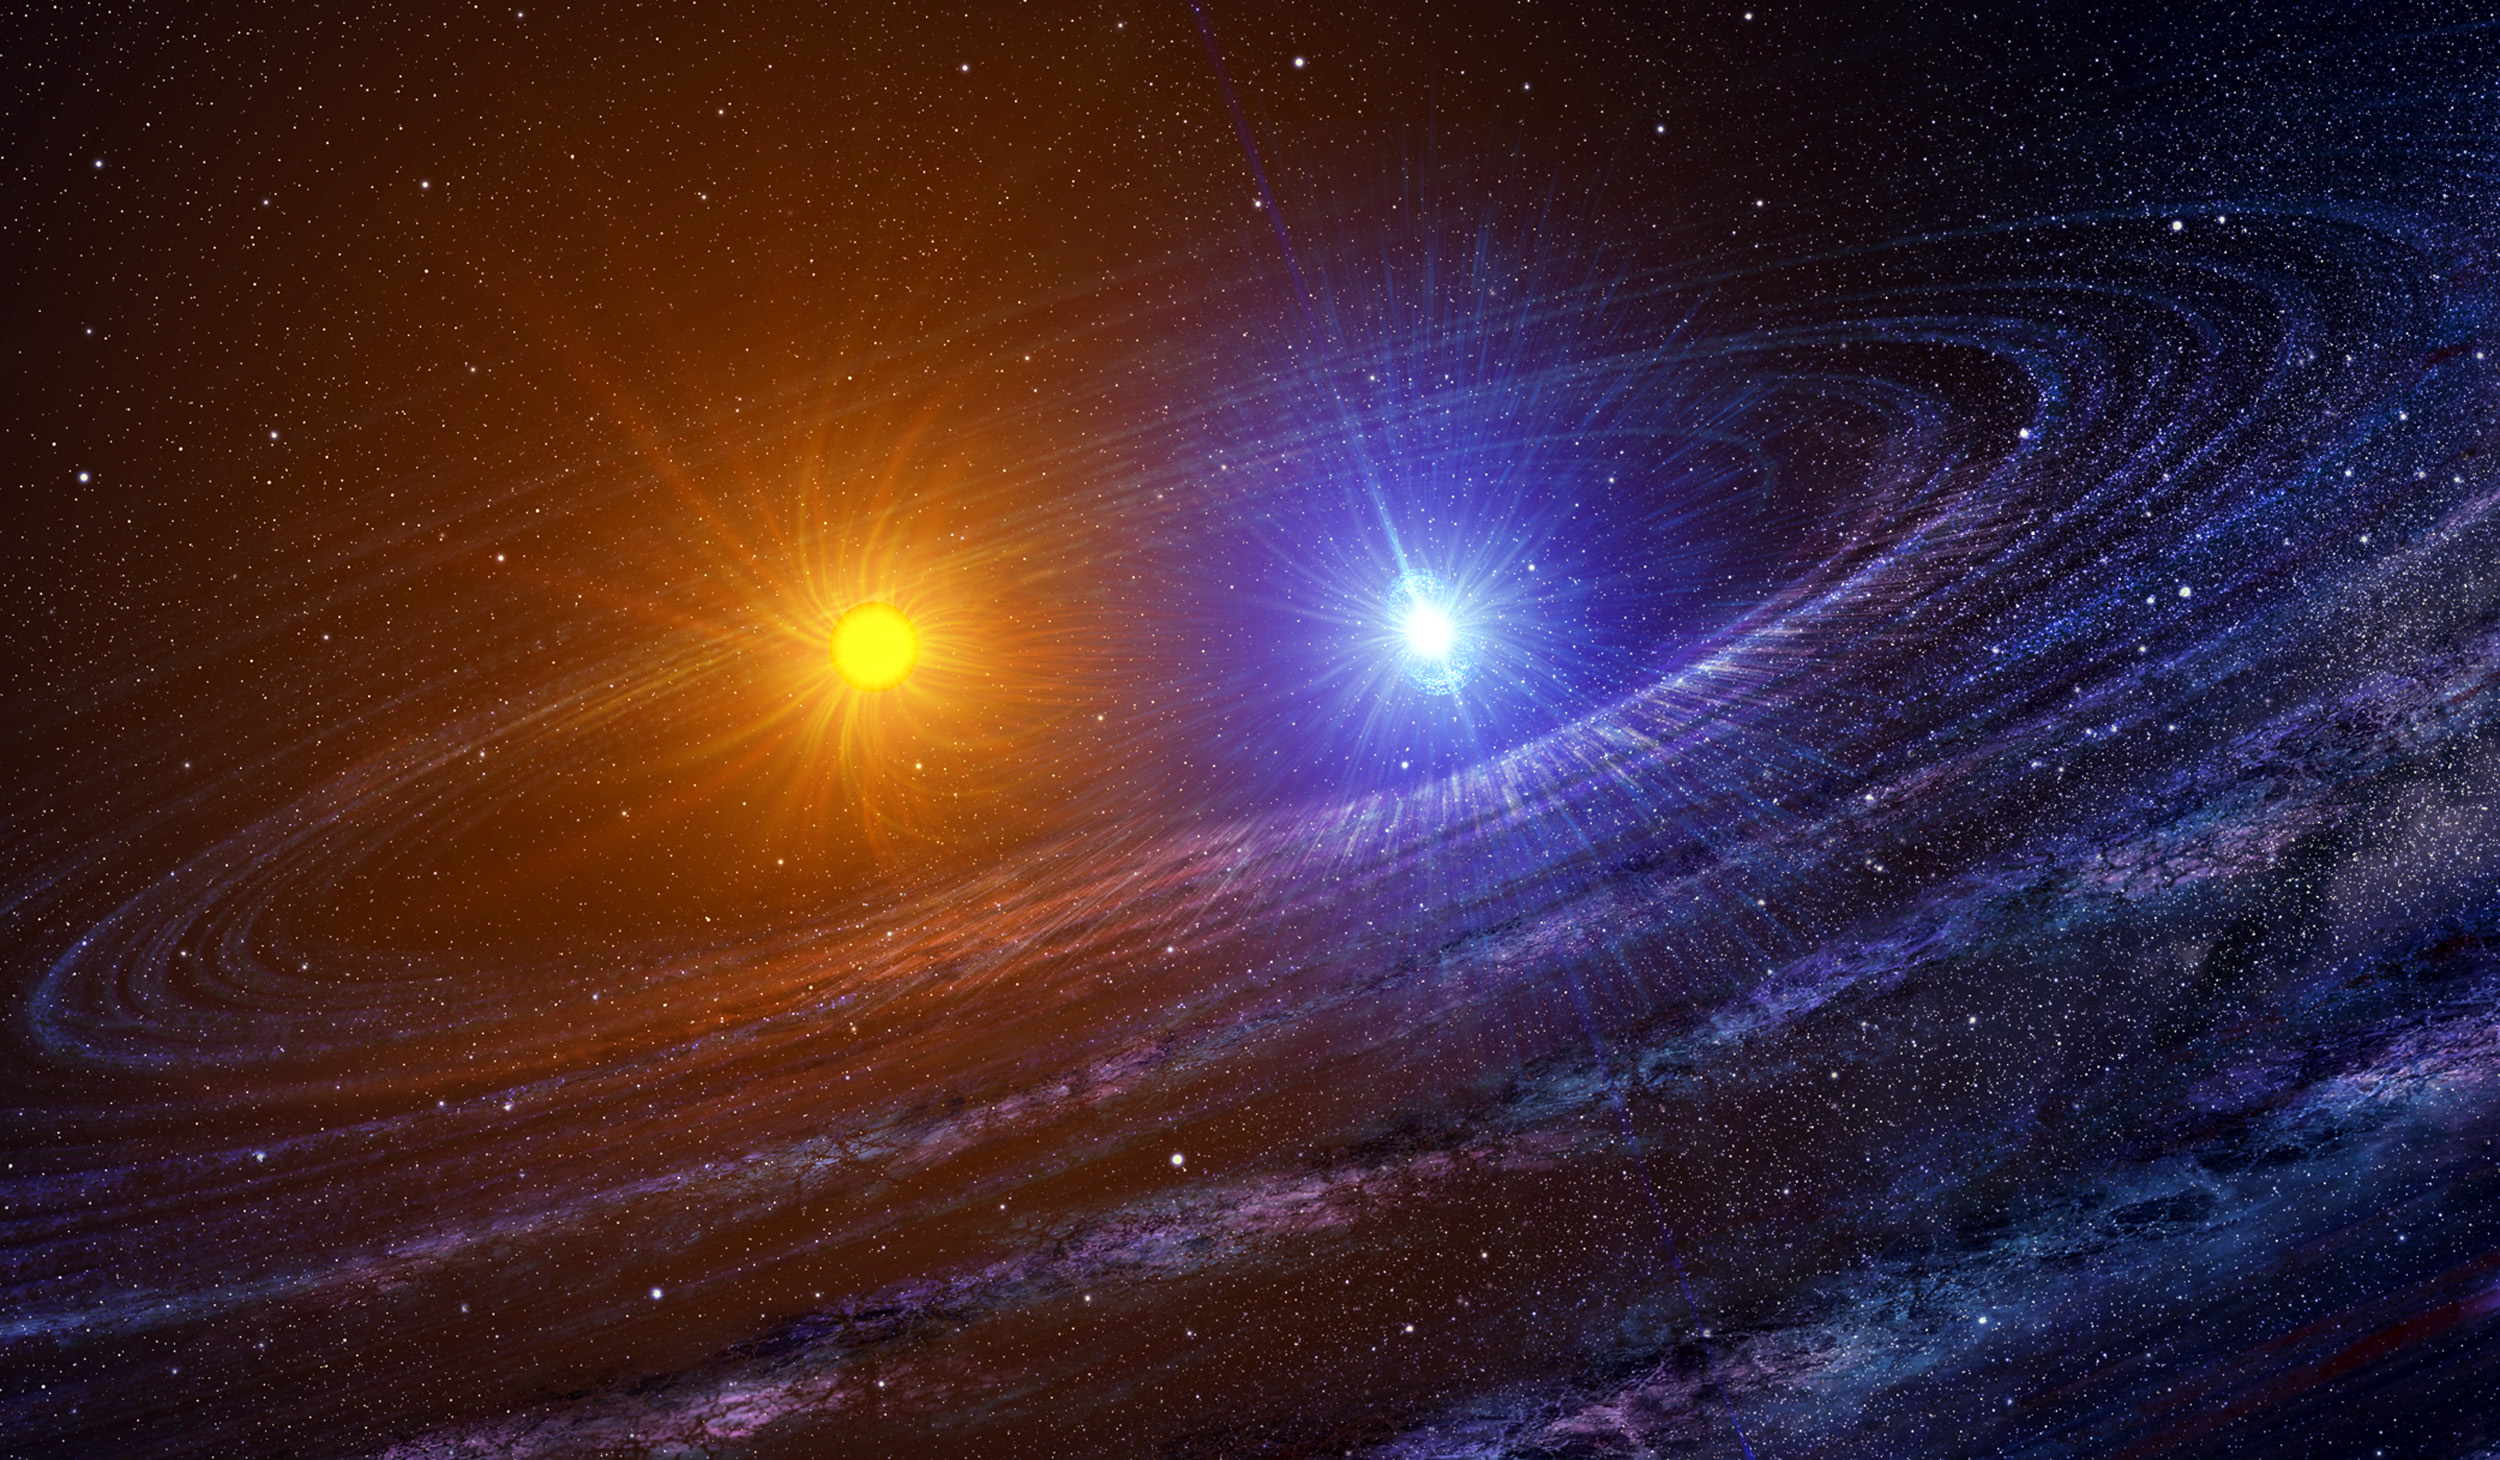
\includegraphics[width=\columnwidth]{presentazione/ophiuchi_binary_system}
        \caption{Crediti: W. M. Keck Observatory}
      \end{figure}
    \end{column}
    \begin{column}{0.48\columnwidth}
      \begin{figure}
        \centering
        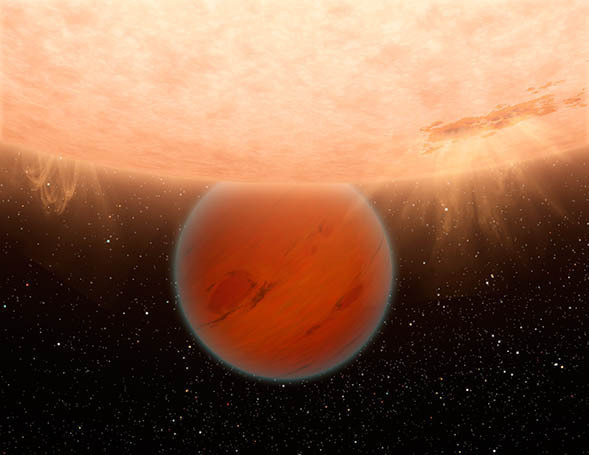
\includegraphics[width=\columnwidth]{presentazione/star-planet}
        \caption{Crediti: NASA/JPL-Caltech}
      \end{figure}
    \end{column}
  \end{columns}
\end{frame}

\begin{frame}
  \frametitle{Risultati del problema dei due corpi}
  \begin{itemize}[<+->]
  \item Il moto dei due corpi può essere ricondotto al
    \alert{moto di un solo corpo} in un potenziale esterno
  \item Si \alert{conserva il momento angolare} e il moto dei due corpi si
    svolge in un \alert{piano} \\
    \centering
    \tdplotsetmaincoords{70}{135}
    \begin{tikzpicture}[tdplot_main_coords,scale=2.5,font=\scriptsize]
      \pgfmathsetmacro{\a}{1} % a=1
\pgfmathsetmacro{\e}{0.8} % e=0.8
\pgfmathsetmacro{\b}{\a*sqrt(1-\e*\e)} % b=a*sqrt(1-e^2)
\pgfmathsetmacro{\c}{\a*\e} % c=a*e
\pgfmathsetmacro{\p}{\a*(1-\e*\e)} % p=a*(1-e^2)
\pgfmathsetmacro{\m}{0.3} % massa
\pgfmathsetmacro{\scala}{4} % fattore di scala per il momento angolare

% funzione che restituisce la quantità di moto nel punto di anomalia vera #1
% (valgono sempre le stesse considerazioni: la funzione restituisce valori
% corretti se #1 != 0, 180, 360 e numeri a loro congrui in modulo 360)
\pgfmathdeclarefunction{mv}{1}{\pgfmathparse{\m*sqrt(2/dist(#1)-1/\a)}}
% funzione che restituisce il modulo del momento angolare nel punto di
% anomalia vera #1. (valgono sempre le stesse considerazioni: la funzione
% restituisce valori corretti se #1 != 0, 180, 360 e numeri a loro congrui
% in modulo 360)
\pgfmathdeclarefunction{momang}{1}%
                      {\pgfmathparse{dist(#1)*mv(#1)*sin(alpha(#1))*\scala}}

%% parametri del primo punto
% anomalia vera del primo punto
\pgfmathsetmacro{\anomaliauno}{0}
% coordinata x del primo punto in cui disegno il vettore posizione
\pgfmathsetmacro{\xuno}{dist(\anomaliauno)*cos(\anomaliauno)}
% coordinata y del primo punto in cui disegno il vettore posizione
\pgfmathsetmacro{\yuno}{dist(\anomaliauno)*sin(\anomaliauno)}
% componente x del vettore quantità di moto. poiché anomalia = 0 pongo
% manualmente p_x = 0, p_y = |p| (negli altri casi posso usare le funzioni
% sopra definite)
\pgfmathsetmacro{\pxuno}{0}
% componente y del vettore quantità di moto
\pgfmathsetmacro{\pyuno}{mv(\anomaliauno)}
%% secondo punto
% anomalia vera del secondo punto
\pgfmathsetmacro{\anomaliadue}{130}
% coordinata x del secondo punto in cui disegno il vettore posizione
\pgfmathsetmacro{\xdue}{dist(\anomaliadue)*cos(\anomaliadue)}
% coordinata y del secondo punto in cui disegno il vettore posizione
\pgfmathsetmacro{\ydue}{dist(\anomaliadue)*sin(\anomaliadue)}
% componente x del vettore quantità di moto
\pgfmathsetmacro{\pxdue}{mv(\anomaliadue)*cos(beta(\anomaliadue))}
% componente y del vettore quantità di moto
\pgfmathsetmacro{\pydue}{mv(\anomaliadue)*sin(beta(\anomaliadue))}

% origine dei sistemi di riferimento
\node [shape=coordinate](O) at (0,0,0) [label=above right:$O$] {};
\draw[->] (O) -- (1,0,0) node[anchor=north east]{$x$}; % asse x
\draw[->] (O) -- (0,1,0) node[anchor=north west]{$y$}; % asse y
\draw[->] (O) -- (0,0,1) node[anchor=south]{$z$}; % asse z
\draw (-\c,0,0) ellipse ({\a} and \b); % ellisse

%% primo punto
\draw[->,thick] (O) -- node[above] {$\bm{r}$} (\xuno,\yuno); % posizione
% vettore quantità di moto
\draw[->,thick] (\xuno,\yuno) -- node[below] {$\bm{p}$} +(\pxuno,\pyuno);
% vettore momento angolare
\draw[->,thick] (\xuno,\yuno,0) -- node[left] {$\bm{l}_0$}
                +(0,0,{dist(\anomaliauno)*mv(\anomaliauno)*\scala});

% %% secondo punto
\draw[->,thick] (O) -- node[above] {$\bm{r}$} (\xdue,\ydue); % posizione
% vettore quantità di moto
\draw[->,thick] (\xdue,\ydue) -- node[below] {$\bm{p}$} +(\pxdue,\pydue);
% vettore momento angolare
\draw[->,thick] (\xdue,\ydue,0) -- node[right] {$\bm{l}_0$}
                +(0,0,{momang(\anomaliadue)});

%%% Local Variables:
%%% mode: latex
%%% TeX-master: "../../tesi"
%%% End:

    \end{tikzpicture}
  \item È valida la \alert{seconda legge di Keplero}
  \end{itemize}
\end{frame}

\begin{frame}
  \frametitle{Equazione dell'orbita nel problema di Keplero}
  L'equazione dell'orbita è
  \begin{equation*}
    r(\theta) = \frac{p}{1 + e \cos\theta}
  \end{equation*}
cioè l'equazione in coordinate polari di una conica (circonferenza, ellisse,
parabola, iperbole). Nel caso dell'ellisse e della circonferenza abbiamo la
\alert{prima legge di Keplero}.
\end{frame}

\begin{frame}
  \frametitle{Ellisse}
  \begin{tikzpicture}[scale=4.5,font=\tiny]
    \pgfmathsetmacro{\a}{1} % a=1
\pgfmathsetmacro{\e}{0.8} % e=0.8
\pgfmathsetmacro{\b}{\a*sqrt(1-\e*\e)} % b=a*sqrt(1-e^2)
\pgfmathsetmacro{\c}{\a*\e} % c=a*e
\pgfmathsetmacro{\p}{\a*(1-\e*\e)} % p=a*(1-e^2)

\draw[->] (-1.1,0) -- (1.1,0) node[right] {$x\equiv x'$}; %assi x e x'
\draw[->] (0,-0.7) -- (0,0.7) node[above] {$y'$}; %asse y'
\draw[->] (\c,-0.7) -- (\c,0.7) node[above] {$y$}; %asse y
\draw[thick] (0,0) ellipse ({\a} and \b); % ellisse
\draw[fill=black] (-\c,0) circle (0.005) node[below] {$F_2$}; % fuoco F_2
\draw (0,0) node[below left] {$O'$}; % origine O'
\draw[fill=black] (\c,0) circle (0.005) % fuoco F_1 e origine O
                  node[below left] {$O\equiv F_1$};
% arco dell'anomalia vera
\draw[->] (\c+0.1,0) to [out=90,in=-45] node[inner sep=0,fill=white,right=3]
          {$\theta$} ($(\c,0) + 0.1*({cos(45)},{sin(45)})$);
\draw[->] (\c,0) -- node[above] {$r$} +($dist(45)*({cos(45},{sin(45)})$);
\draw[<->] (0,0.04) -- node[above] {$a$} +(-\a,0);
\draw[<->] (0,0.04) -- node[above] {$c$} +(\c,0);
\draw[<->] (-0.04,0) -- node[left] {$b$} +(0,\b);
\draw[<->] (\c-0.04,0) -- node[left] {$p$} +(0,\p);
\draw[<->] (\c,-0.04) -- node[below] {$a-c$} +({\a-\c},0);

%%% Local Variables:
%%% mode: latex
%%% TeX-master: "../../presentazione"
%%% End:

  \end{tikzpicture}
\end{frame}

% % non metto questa slide, non è necessaria
% \begin{frame}
%   \frametitle{Geometria del sistema binario}
%   \begin{center}
%     \tdplotsetmaincoords{70}{135}
%     \begin{tikzpicture}[tdplot_main_coords,scale=4.5,font=\tiny]
%       %% colori
% colore per gli assi del sistema di riferimento Ox'y'z'
\colorlet{intrinseco}{black}
% colore per gli assi del sistema di riferimento Oxyz
\colorlet{ausiliario}{red}
% colore per gli assi del sistema di riferimento Ox'y'z'
\colorlet{pdc}{blue}

\pgfmathsetmacro{\angolophi}{20} % valore dell'angolo `phi_0'
\pgfmathsetmacro{\angoloi}{40} % valore dell'angolo `i'
% origine dei sistemi di riferimento
\node [shape=coordinate](O) at (0,0,0) [label=above right:$O$] {};
% asse x'
\draw[->,intrinseco] (O) -- (1,0,0) node[anchor=north east]{$x'$};
% asse y'
\draw[->,intrinseco] (O) -- (0,1,0) node[anchor=north west]{$y'$};
% asse z' (coincidente con l'asse z)
\draw[->,intrinseco!50!ausiliario] (O) -- (0,0,1) node[anchor=south]{$z'
  \equiv z$};
\draw[thick] (-0.4,0,0) ellipse (0.5 and 0.3); % ellisse

% ruoto il sistema di riferimento principale x'y'z' intorno all'asse z'
% dell'angolo `phi_0'
\tdplotsetrotatedcoords{\angolophi}{0}{0}
% asse x
\draw[tdplot_rotated_coords,->,ausiliario] (O) -- (1,0,0)
                                           node[anchor=north]{$x$};
% asse y (coincidente con l'asse y'')
\draw[tdplot_rotated_coords,->,ausiliario!50!pdc] (O) -- (0,1,0)
                                           node[anchor=west]{$y \equiv y''$};
% disegno archi dell'angolo `phi_0'
\tdplotdrawarc[->,tdplot_rotated_coords,ausiliario]{(O)}{0.8}{-\angolophi}%
{0}{anchor=north east}{$\phi_0$}
\tdplotdrawarc[->,tdplot_rotated_coords,ausiliario]{(O)}{0.8}%
{90-\angolophi}{90}{anchor=north west}{$\phi_0$}

% ruoto il sistema di riferimento xyz (che deriva a sua volta dalla rotazione di
% x'y'z' attorno a z' dell'angolo `phi_0') intorno all'asse y dell'angolo `i'
\tdplotsetrotatedcoords{\angolophi}{-\angoloi}{0}
% asse x''
\draw[tdplot_rotated_coords,->,pdc] (O) -- (1,0,0)
                                    node[anchor=east]{$x''$};
% asse z''
\draw[tdplot_rotated_coords,->,pdc] (O) -- (0,0,1)
                                    node[anchor=south]{$z''$};
% ruoto il piano theta (di `phi_0') per disegnare l'arco di `i'
\tdplotsetthetaplanecoords{\angolophi}
% disegno archi dell'angolo `i' e `pi/2-i'
\tdplotdrawarc[->,tdplot_rotated_coords,pdc]{(O)}{0.8}{90-\angoloi}%
{0}{anchor=south east}{$i$}
\tdplotdrawarc[->,tdplot_rotated_coords,pdc]{(O)}{0.8}{90}%
{90-\angoloi}{anchor=south east}{$\pi/2-i$}
\tdplotdrawarc[->,tdplot_rotated_coords,pdc]{(O)}{0.8}{0}%
{-\angoloi}{anchor=south}{$\pi/2-i$}

%%% Local Variables:
%%% mode: latex
%%% TeX-master: "../../tesi"
%%% End:

%     \end{tikzpicture}
%   \end{center}
% \end{frame}

\begin{frame}
  \frametitle{Evoluzione temporale}
  \begin{block}{Equazione di Keplero}
    \begin{equation*}
    \phi(t) \equiv \omega t = \psi(t) - e\sin\psi(t)
  \end{equation*}
  \end{block}
  \begin{center}
    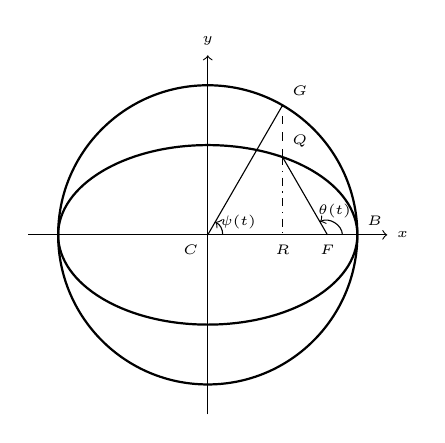
\begin{tikzpicture}[font=\tiny,scale=1.9]
      \pgfmathsetmacro{\a}{1} % a=1
\pgfmathsetmacro{\e}{0.8} % e=0.8
\pgfmathsetmacro{\b}{\a*sqrt(1-\e*\e)} % b=a*sqrt(1-e^2)
\pgfmathsetmacro{\c}{\a*\e} % c=a*e
\pgfmathsetmacro{\p}{\a*(1-\e*\e)} % p=a*(1-e^2)
\pgfmathsetmacro{\anomalia}{120} % theta=120
% r(theta)=p/(1+e*cos(theta))
\pgfmathsetmacro{\r}{\p/(1+\e*cos(\anomalia))}
\pgfmathsetmacro{\xq}{\c+\r*cos(\anomalia)} % x_Q=x_G=c+r(theta)*cos(theta)
\pgfmathsetmacro{\yq}{\r*sin(\anomalia)} % y_Q=r(theta)*sin(theta)
\pgfmathsetmacro{\yg}{\yq*\a/\b} % y_G=y_Q*a/b
% calcolo anomalia eccentrica (da relazione fra anomalia vera ed eccentrica)
\pgfmathsetmacro{\angolopsi}{2*atan(sqrt((1-\e)/(1+\e))*tan(\anomalia/2))}

\draw [->] (-1.2,0) -- (1.2,0) node[right] {$x$}; %asse x
\draw [->] (0,-1.2) -- (0,1.2) node[above] {$y$}; %asse y
\draw[thick] (0,0) circle (\a); % circonferenza ausiliaria
\draw[thick] (0,0) ellipse ({\a} and \b); %ellisse
\draw (\c,0) -- (\xq,\yq) node[above right] {$Q$}; % segmento FQ
\draw [dashed] (\xq,\yq) -- (\xq,\yg); % segmento QG
\draw (0,0) -- (\xq,\yg) node[above right] {$G$}; % segmento CG
\draw (0,0) node[below left] {$C$}; % etichetta del punto C
\draw (\c,0) node[below] {$F$}; % etichetta del punto F
\draw (\a,0) node[above right] {$B$}; % etichetta del punto B
\draw [dashdotted] (\xq,\yq) -- (\xq,0) node[below] {$R$}; % segmento RQ
% angolo theta (anomalia vera(
\draw [->] (\c+0.1,0) to [out=90,in=\anomalia-90] node[above=-2] {$\theta(t)$}
           ($(\c,0)+cos(\anomalia)*(0.1,0) + sin(\anomalia)*(0,0.1)$);
% angolo psi (anomalia eccentrica)
\draw [->] (0.1,0) to [out=90,in=\angolopsi-90] node[above right=-4] {$\psi(t)$}
           ($(0,0)+cos(\angolopsi)*(0.1,0)+sin(\angolopsi)*(0,0.1)$);

%%% Local Variables:
%%% mode: latex
%%% TeX-master: "../../tesi"
%%% End:

    \end{tikzpicture}
  \end{center}
\end{frame}

\begin{frame}
  \frametitle{Applicazioni: Sgr A*}
  \begin{adv}
  \item Stima della massa di corpi non visibili
  \end{adv}
  \begin{figure}
    \centering
    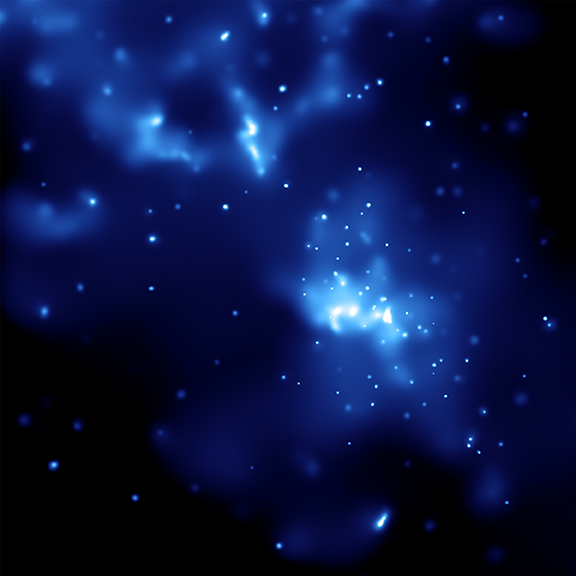
\includegraphics[width=0.49\columnwidth]{presentazione/sgra}
    \caption{Crediti: NASA/CXC/SAO}
  \end{figure}
\end{frame}

\begin{frame}
  \frametitle{Applicazioni: Sgr A* (continua)}
  \begin{columns}
    \begin{column}{0.4\columnwidth}
      \begin{table}
        \centering
        \begin{tabular}{lc}
          \toprule
          Grandezza         & Valore                       \\
          \midrule
          $R_0$             & \SI{7.96}{\kilo\parsec}      \\
          $P$               & \SI{15.86}{\year}            \\
          $a$               & \SI{126.5}{\milli\arcsecond} \\
          $e$               & $0.8904$                     \\
          $R_\textup{min}$  & \SI{0.535}{\milli\parsec}    \\
          $M_{\textup{S}2}$ & circa \SI{15}{\solarmass}    \\
          \bottomrule
        \end{tabular}
      \end{table}
      Con questi dati $M_{\textup{BH}} = \SI{4.06e6}{\solarmass}$.
    \end{column}
    \begin{column}{0.5\columnwidth}
      \begin{figure}
        \centering
        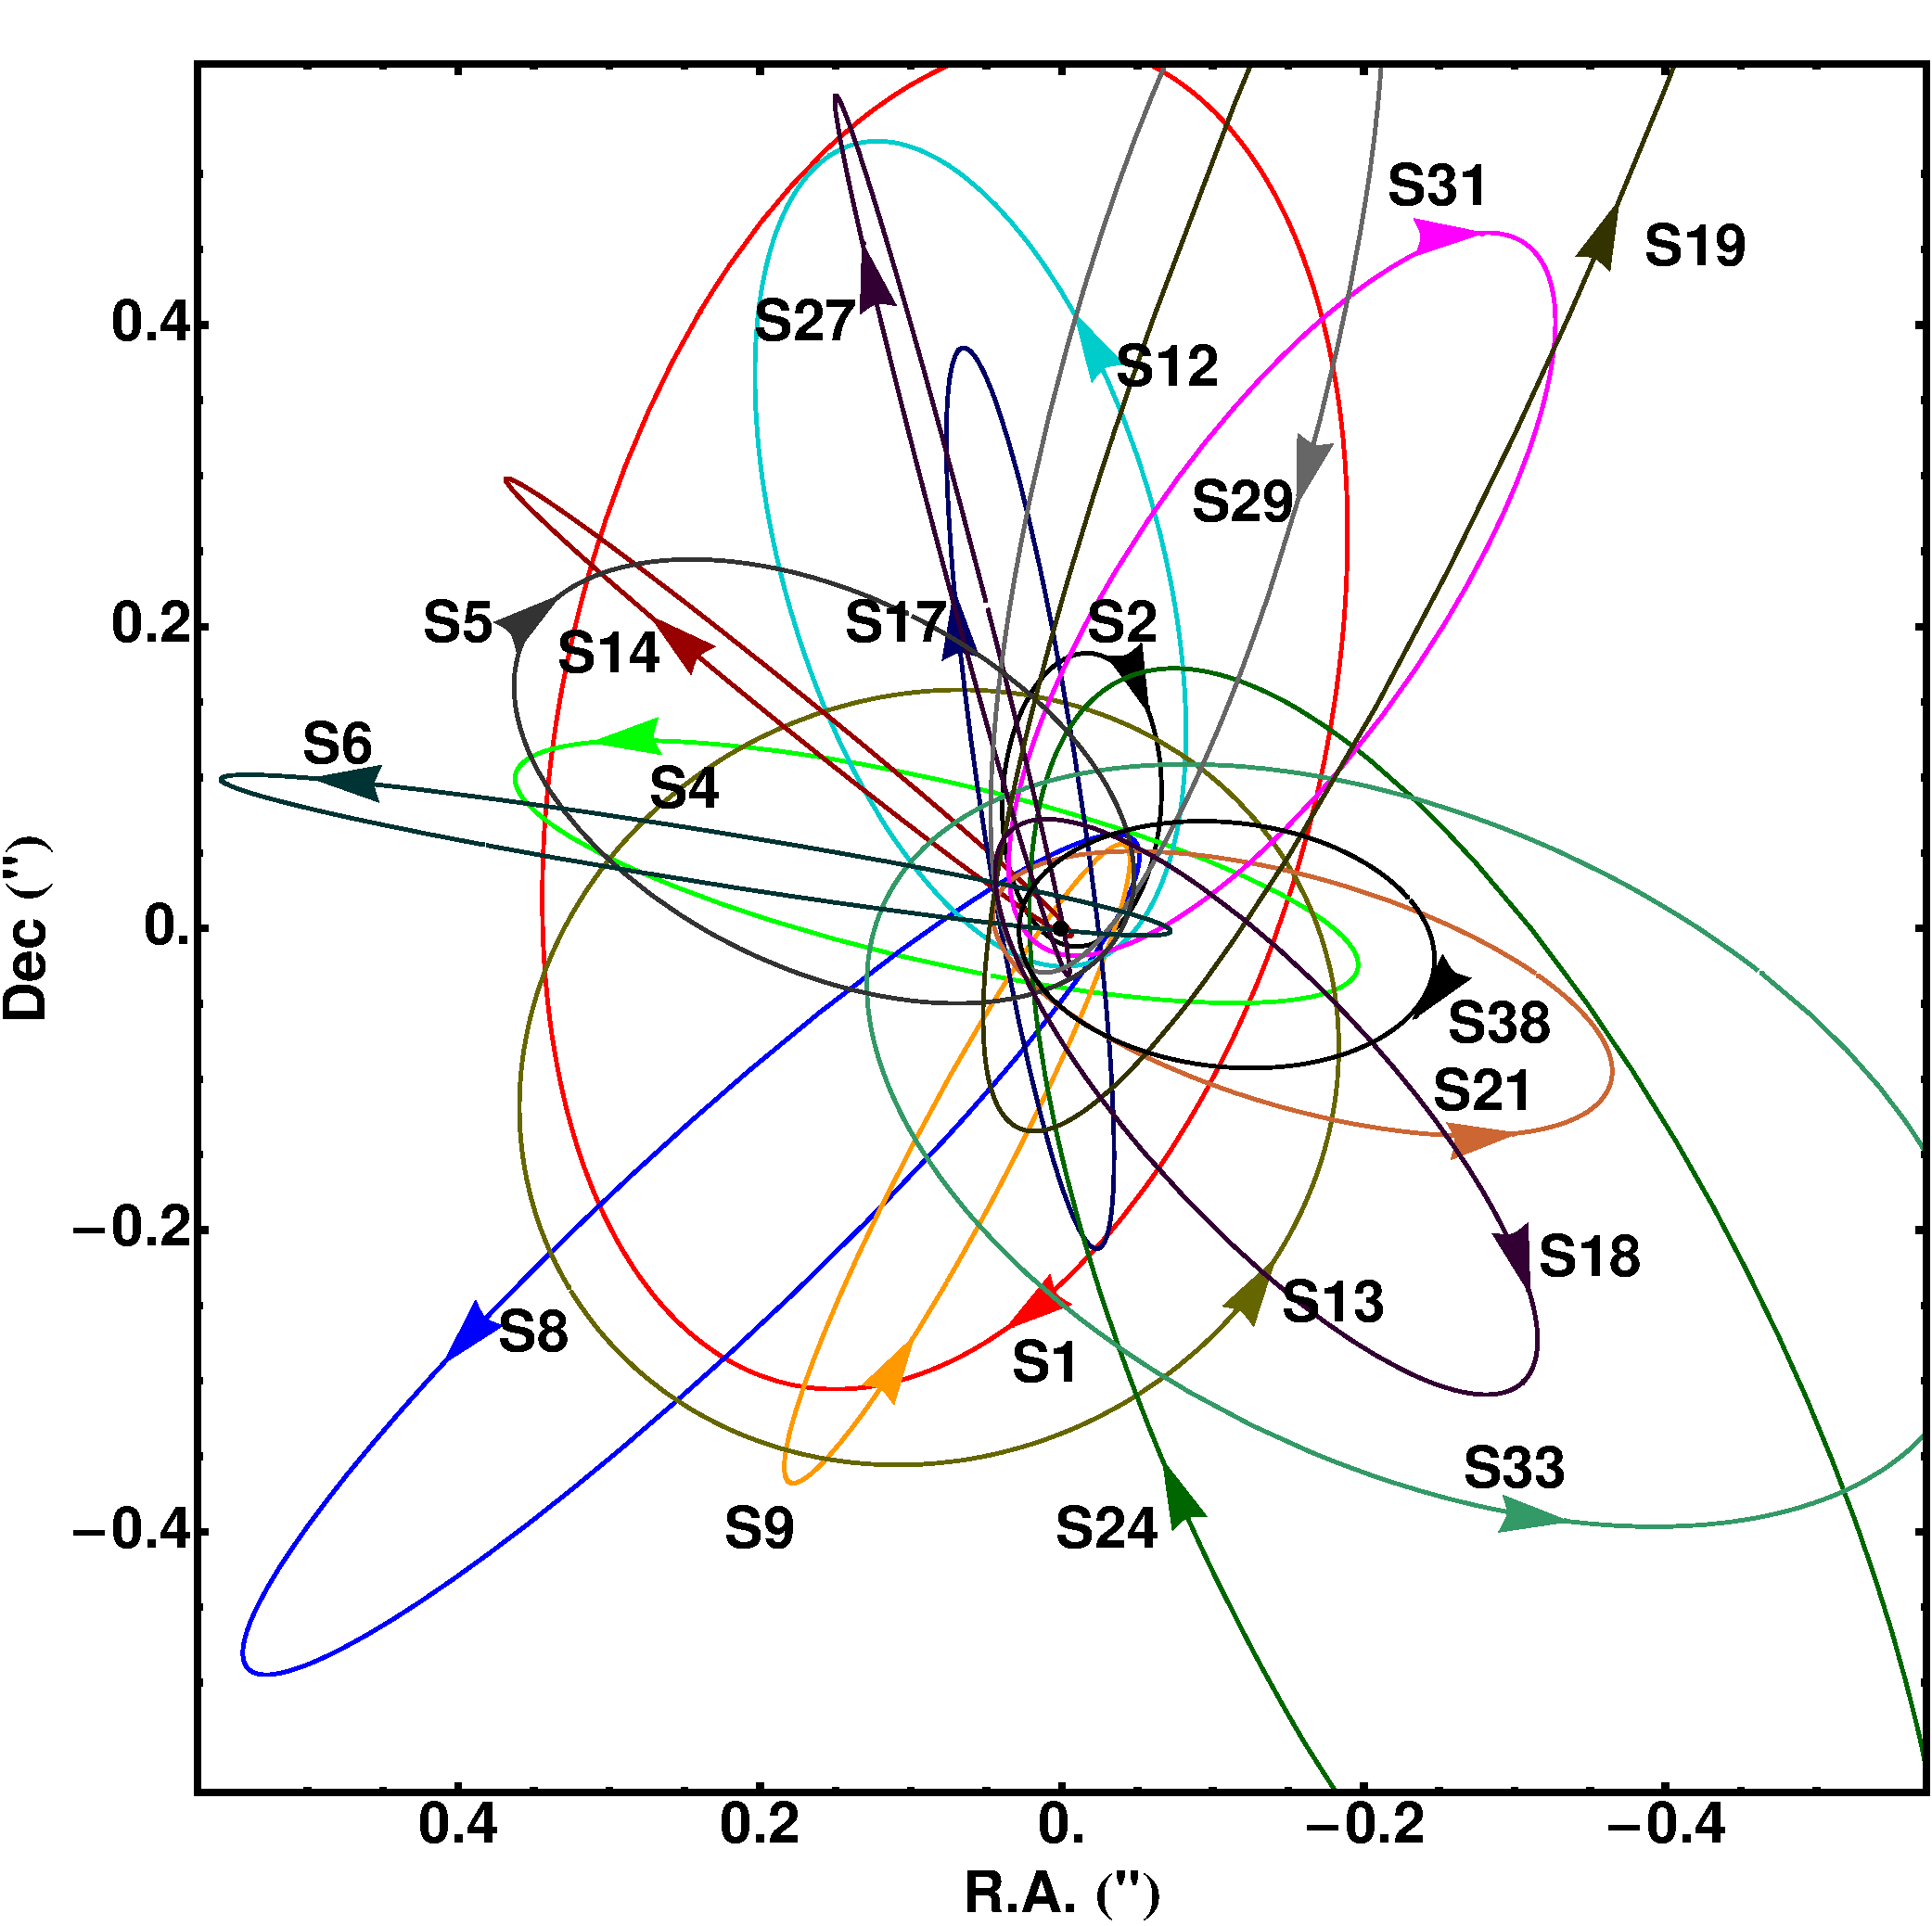
\includegraphics[width=\columnwidth]{orbite_sgra}
        \caption{Crediti: S. Gillessen \emph{et al}}
      \end{figure}
    \end{column}
  \end{columns}
\end{frame}

\begin{frame}
  \frametitle{Applicazioni: Cygnus X-1}
  \begin{columns}
    \begin{column}{0.35\columnwidth}
      Funzione di massa
      \begin{equation*}
        f(m_{1},m_{2}) = \frac{v_{1}^{3}P}{2\pi G}
      \end{equation*}
      Dati noti \\
      $P = \SI{5.6}{d},$ \\
      $v_{1} = \SI{75}{\kilo\metre\per\second}$. \\
      Risultato \\
      $m_{2} \gtrsim \SI{4}{\solarmass}$.
    \end{column}
    \begin{column}{0.55\columnwidth}
      \begin{figure}
        \centering
        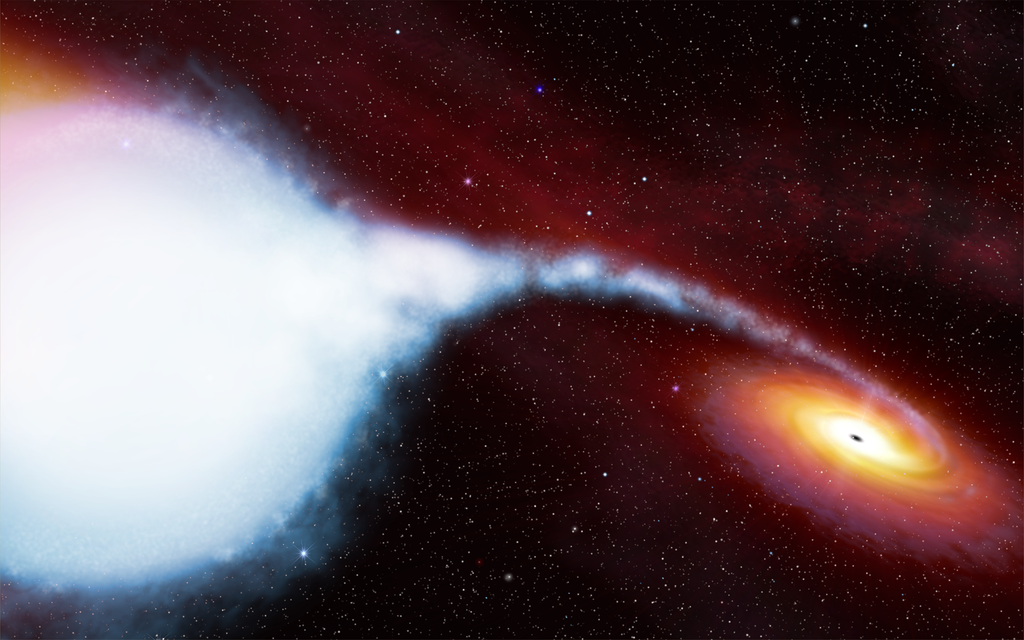
\includegraphics[width=\columnwidth]{presentazione/cygnusx1}
        \caption{Crediti: ESA/Hubble}
    \end{figure}
    \end{column}
  \end{columns}
\end{frame}

\begin{frame}
  \frametitle{Applicazioni: transiti}
  \begin{adv}
  \item Individuazione e studio di pianeti extrasolari
  \end{adv}
  \begin{figure}
    \centering
    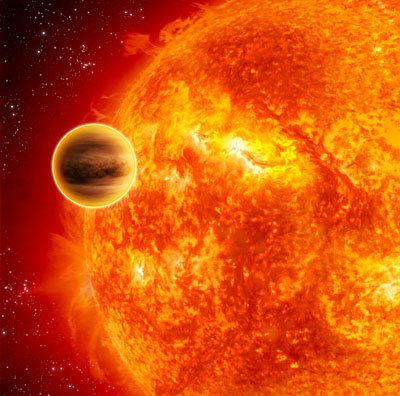
\includegraphics[width=0.5\columnwidth]{presentazione/transit}
    \caption{Crediti: NASA/JPL-Caltech}
  \end{figure}
\end{frame}

\begin{frame}
  \frametitle{Applicazioni: transiti (continua)}
  $\Delta t = t_{\textup{ef}} - t_{ii} = \dfrac{P(r_{1} + r_{2})}{\pi a}$
  \begin{center}
    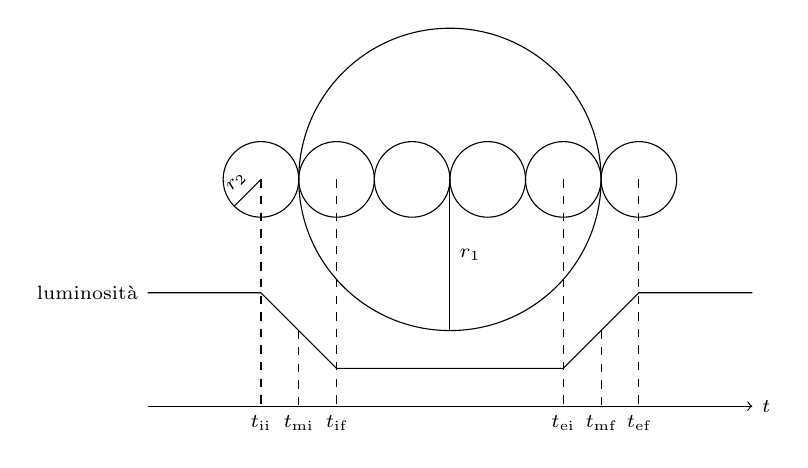
\begin{tikzpicture}[scale=0.48,font=\scriptsize]
      \pgfmathsetmacro{\rdue}{1} % raggio pianeta = 1
\pgfmathsetmacro{\runo}{4*\rdue} % raggio stella = 4

\coordinate (O) at (0,0); % centro stella
\draw (O) circle (\runo); % disco stella
\draw (O) -- node[right] {$r_1$} +(0,-\runo);
\draw (-\runo-\rdue,0) -- node[above,sloped] {$r_2$}
      +($-\rdue*({cos(45)},{sin(45)})$);
\foreach \x in {-5,-3,-1,1,3,5} % varie posizioni del pianeta
  \draw (\x,0) circle (\rdue);
\draw (-8,-\runo+1) node[left] {luminosità} -- (-\runo-\rdue,-\runo+1) --
      (-\runo+\rdue,-\runo-1) -- (\runo-1,-\runo-1) --
      (\runo+\rdue,-\runo+1) -- (8,-\runo+1); % curva di luce
\draw[dashed] (-\runo-\rdue,0) -- (-\runo-\rdue,-\runo-2) node[below]
              {$t_{\textup{ii}}$};
\draw[dashed] (-\runo,-\runo) -- (-\runo,-\runo-2) node[below]
              {$t_{\textup{mi}}$};
\draw[dashed] (-\runo+\rdue,0) -- (-\runo+\rdue,-\runo-2) node[below]
              {$t_{\textup{if}}$};
\draw[dashed] (\runo-\rdue,0) -- (\runo-\rdue,-\runo-2) node[below]
              {$t_{\textup{ei}}$};
\draw[dashed] (\runo,-\runo) -- (\runo,-\runo-2) node[below]
              {$t_{\textup{mf}}$};
\draw[dashed] (\runo+\rdue,0) -- (\runo+\rdue,-\runo-2) node[below]
              {$t_{\textup{ef}}$};
\draw[->] (-8,-\runo-2) -- (8,-\runo-2) node[right] {$t$}; % asse del tempo

%%% Local Variables:
%%% mode: latex
%%% TeX-master: "../../tesi"
%%% End:

    \end{tikzpicture}
  \end{center}
\end{frame}

\begin{frame}
  \frametitle{Applicazioni: transiti (continua)}
  \begin{columns}
    \begin{column}{0.35\columnwidth}
      \begin{figure}
        \centering
        \begin{tikzpicture}[scale=0.55]
          \begin{axis}[restrict x to domain=0.985:1.005,xlabel={Fase
              orbitale},ylabel={luminosità},
            xtick={0.985,0.99,0.995,1,1.005},
            xticklabels={$0.985$,$0.990$,$0.995$,$1.000$,$1.005$},
            ytick={0.99,0.995,1,1.005},
            yticklabels={$0.990$,$0.995$,$1.000$,$1.005$}]
            \addplot[mark=none]
            table[x index=0,y index=8]{programmi/eclissi.dat};
          \end{axis}
        \end{tikzpicture}
      \end{figure}
    \end{column}
    \begin{column}{0.55\columnwidth}
      \begin{figure}
        \centering
        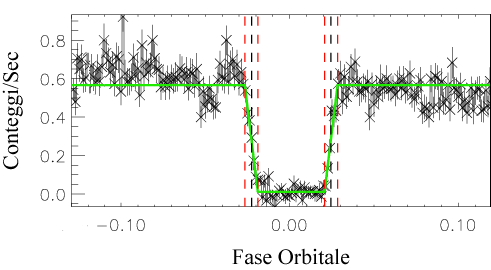
\includegraphics[width=0.95\columnwidth]{presentazione/transito_nucita}
        \caption{Crediti: Nucita \emph{et al}}
      \end{figure}
    \end{column}
  \end{columns}
\end{frame}

\begin{frame}
  \frametitle{Applicazioni: velocità radiale}
  \begin{adv}
  \item Calcolo della velocità di allontanamento dei sistemi binari
    % ricorda che con questa tecnica si può anche stimare il rapporto fra le
    % masse dei due corpi
  \end{adv}
  \begin{figure}
    \centering
    \begin{tikzpicture}[scale=0.9]
      \begin{axis}[xlabel=$\theta$,
  ylabel={$v_{\textup{los}}(\theta)$ (\si{\kilo\metre\per\second})},
  legend pos=north west]
  % l'opzione `raw gnuplot' serve per permettere di scrivere uno script
  % gnuplot come argomento di `\addplot'. È una funzione molto comoda ma
  % mal documentata in pgfplots.
  \addplot [raw gnuplot,mark=none,red] gnuplot {
    r(a,e,x)=a*(1-e**2)/(1+e*cos(x));
    GM=5e11;
    v(a,e,x)=sqrt(GM*(2./r(a,e,x)-1/a));
    alpha(x,e)= e==0 ? pi/2 : ((x<=pi) ? atan(1/tan(x)+1/(e*sin(x))) :
                                         atan(1/tan(x)+1/(e*sin(x)))-pi);
    beta(x,e)= e==0 ? x+pi/2 : x+alpha(x,e);
    vlos(a,e,x)=v(a,e,x)*(cos(beta(x,e)));
    a=5e7;
    e=0.5;
    m1=5.0;
    m2=1.0;
    mu=m1*m2/(m1+m2);
    plot [0.001:2*pi] -mu/m1*vlos(a,e,x)-50
  };
  \addplot [raw gnuplot,mark=none,blue] gnuplot {
    r(a,e,x)=a*(1-e**2)/(1+e*cos(x));
    GM=5e11;
    v(a,e,x)=sqrt(GM*(2./r(a,e,x)-1/a));
    alpha(x,e)= e==0 ? pi/2 : ((x<=pi) ? atan(1/tan(x)+1/(e*sin(x))) :
                                         atan(1/tan(x)+1/(e*sin(x)))-pi);
    beta(x,e)= e==0 ? x+pi/2 : x+alpha(x,e);
    vlos(a,e,x)=v(a,e,x)*(cos(beta(x,e)));
    a=5e7;
    e=0.5;
    m1=5.0;
    m2=1.0;
    mu=m1*m2/(m1+m2);
    plot [0.001:2*pi] mu/m2*vlos(a,e,x)-50
  };
  \legend{$m_{1}$,$m_{2}$}
\end{axis}

%%% Local Variables: 
%%% mode: latex
%%% TeX-master: "../../presentazione"
%%% End: 

    \end{tikzpicture}
  \end{figure}
\end{frame}


\end{document}

%%% Local Variables:
%%% mode: latex
%%% TeX-master: t
%%% End:
